\documentclass[12pt, letterpaper]{report}
\usepackage[margin=1in]{geometry}
\usepackage[utf8]{inputenc}
\usepackage{graphicx}
\usepackage{amsmath}
\usepackage{float}
\usepackage{subfig}
\graphicspath{ {./img/} }
\setlength\parindent{0pt}
\renewcommand\thesection{\Roman{section}.}
\renewcommand{\thesubsection}{\alph{subsection}.}


\title{CS1675 - Assignment 5}
\author{Zachary M. Mattis}


\begin{document}
	
\maketitle

\section{Problem 1 - Logistic Regression Model}

% A
\subsection{Normalization}

\begin{verbatim}
    data_normalize.m
\end{verbatim}

% B
\subsection{Batch-Mode Gradient}

\begin{verbatim}
    Log_regression.m
\end{verbatim}


% C
\subsection{Training Gradient}

\begin{verbatim}
    main1.m
\end{verbatim}


% D
\subsection{Misclassification, Confusion, Sensitivity, Specificity}

\begin{table}[H]
	\centering
	\begin{tabular}{ |l|l| }
		\hline
		\textbf{Dataset} & \textbf{Misclassification Error} \\
		\hline
		Training & 0.2988 \\
		\hline
		Testing & 0.2722 \\
		\hline
	\end{tabular}
	\caption{Misclassification Error}
\end{table}

\begin{table}[H]
	\centering
	\begin{tabular}{ |r|l|l| }
		\hline
		\textbf{Predict / Target} & \textbf{1} & \textbf{1} \\
		\hline
		\textbf{1} & 118 & 42 \\
		\hline
		\textbf{0} & 82 & 297 \\
		\hline
	\end{tabular}
	\caption{Training Confusion Matrix}
\end{table}

\begin{table}[H]
	\centering
	\begin{tabular}{ |r|l|l| }
		\hline
		\textbf{Predict / Target} & \textbf{1} & \textbf{1} \\
		\hline
		\textbf{1} & 46 & 27 \\
		\hline
		\textbf{0} & 22 & 134 \\
		\hline
	\end{tabular}
	\caption{Test Confusion Matrix}
\end{table}

\begin{table}[H]
	\centering
	\begin{tabular}{ |l|l| }
		\hline
		Sensitivity & 0.6765 \\
		\hline
		Specificity & 0.8323 \\
		\hline
	\end{tabular}
	\caption{Test Sensitivity / Specificity}
\end{table}

\subsection{Efficiency}

For a $\frac{2}{\sqrt{k}}$ schedule, the gradient converged after 30,000 epochs. For a $\frac{2}{k}$ schedule, the gradient converged after 200 epochs. Differing starting weights of $\pm100$ also converged in the same amount of time, resulting in a test misclassification error of 0.2722 and training error of 0.2988.

\section{Problem 2.1 - Naive Bayes Model}

% A
\subsection{Data Analysis}

\begin{figure}[H]
	\centering
	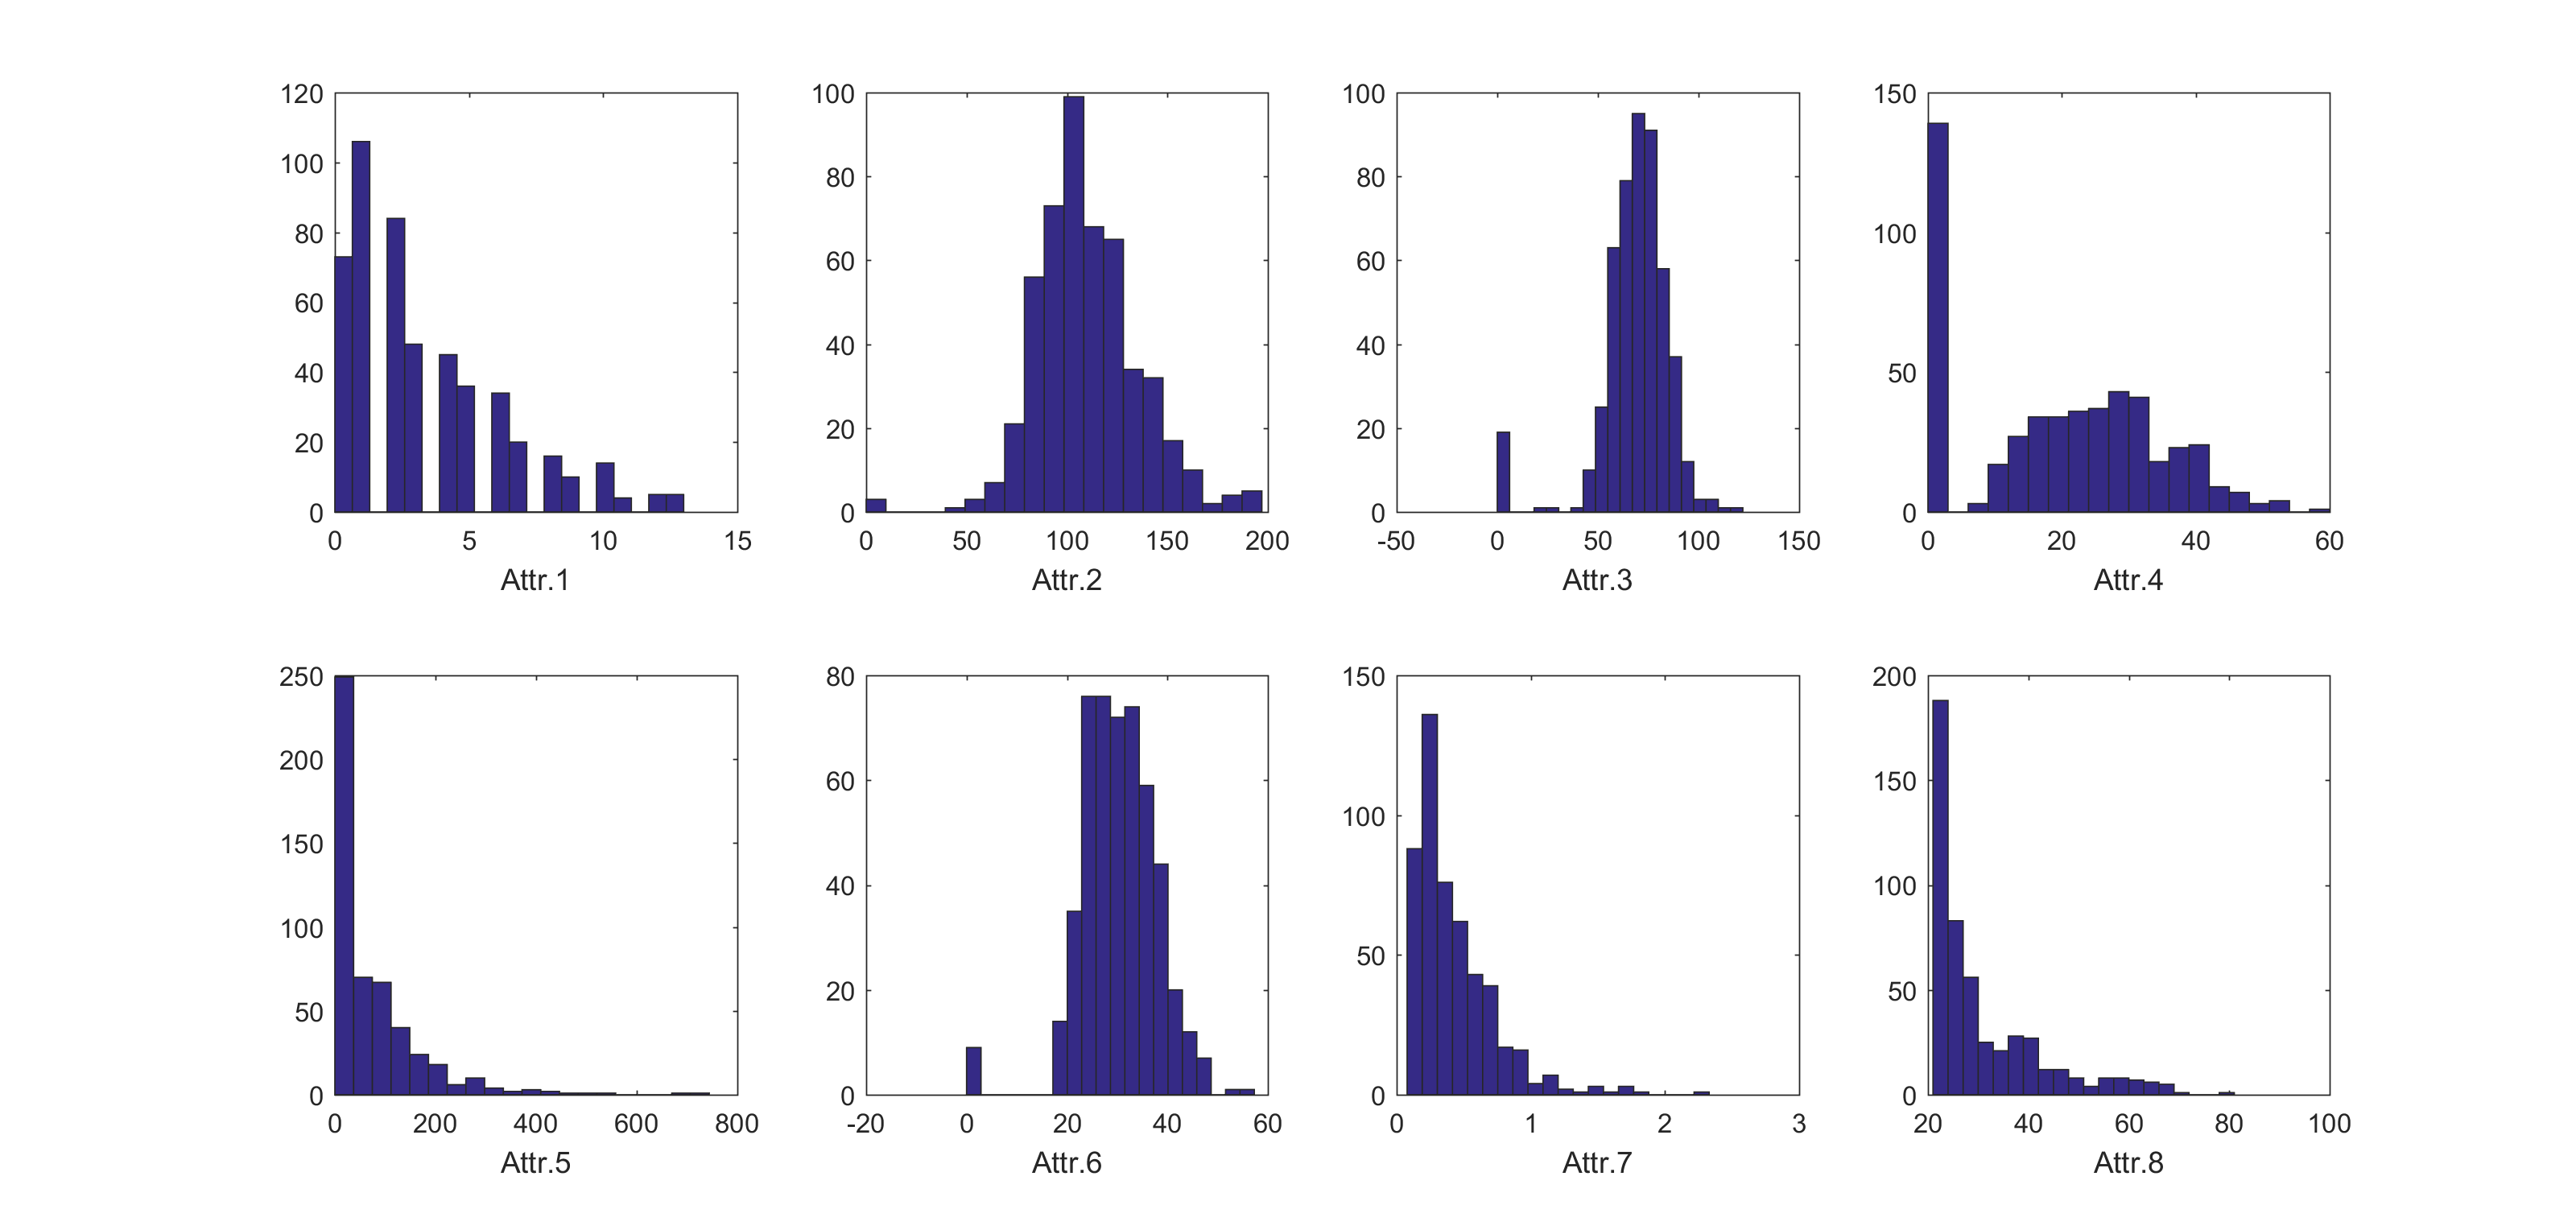
\includegraphics[width=\columnwidth]{p2a0.png}
	\caption{Class 0}
\end{figure}

\begin{figure}[H]
	\centering
	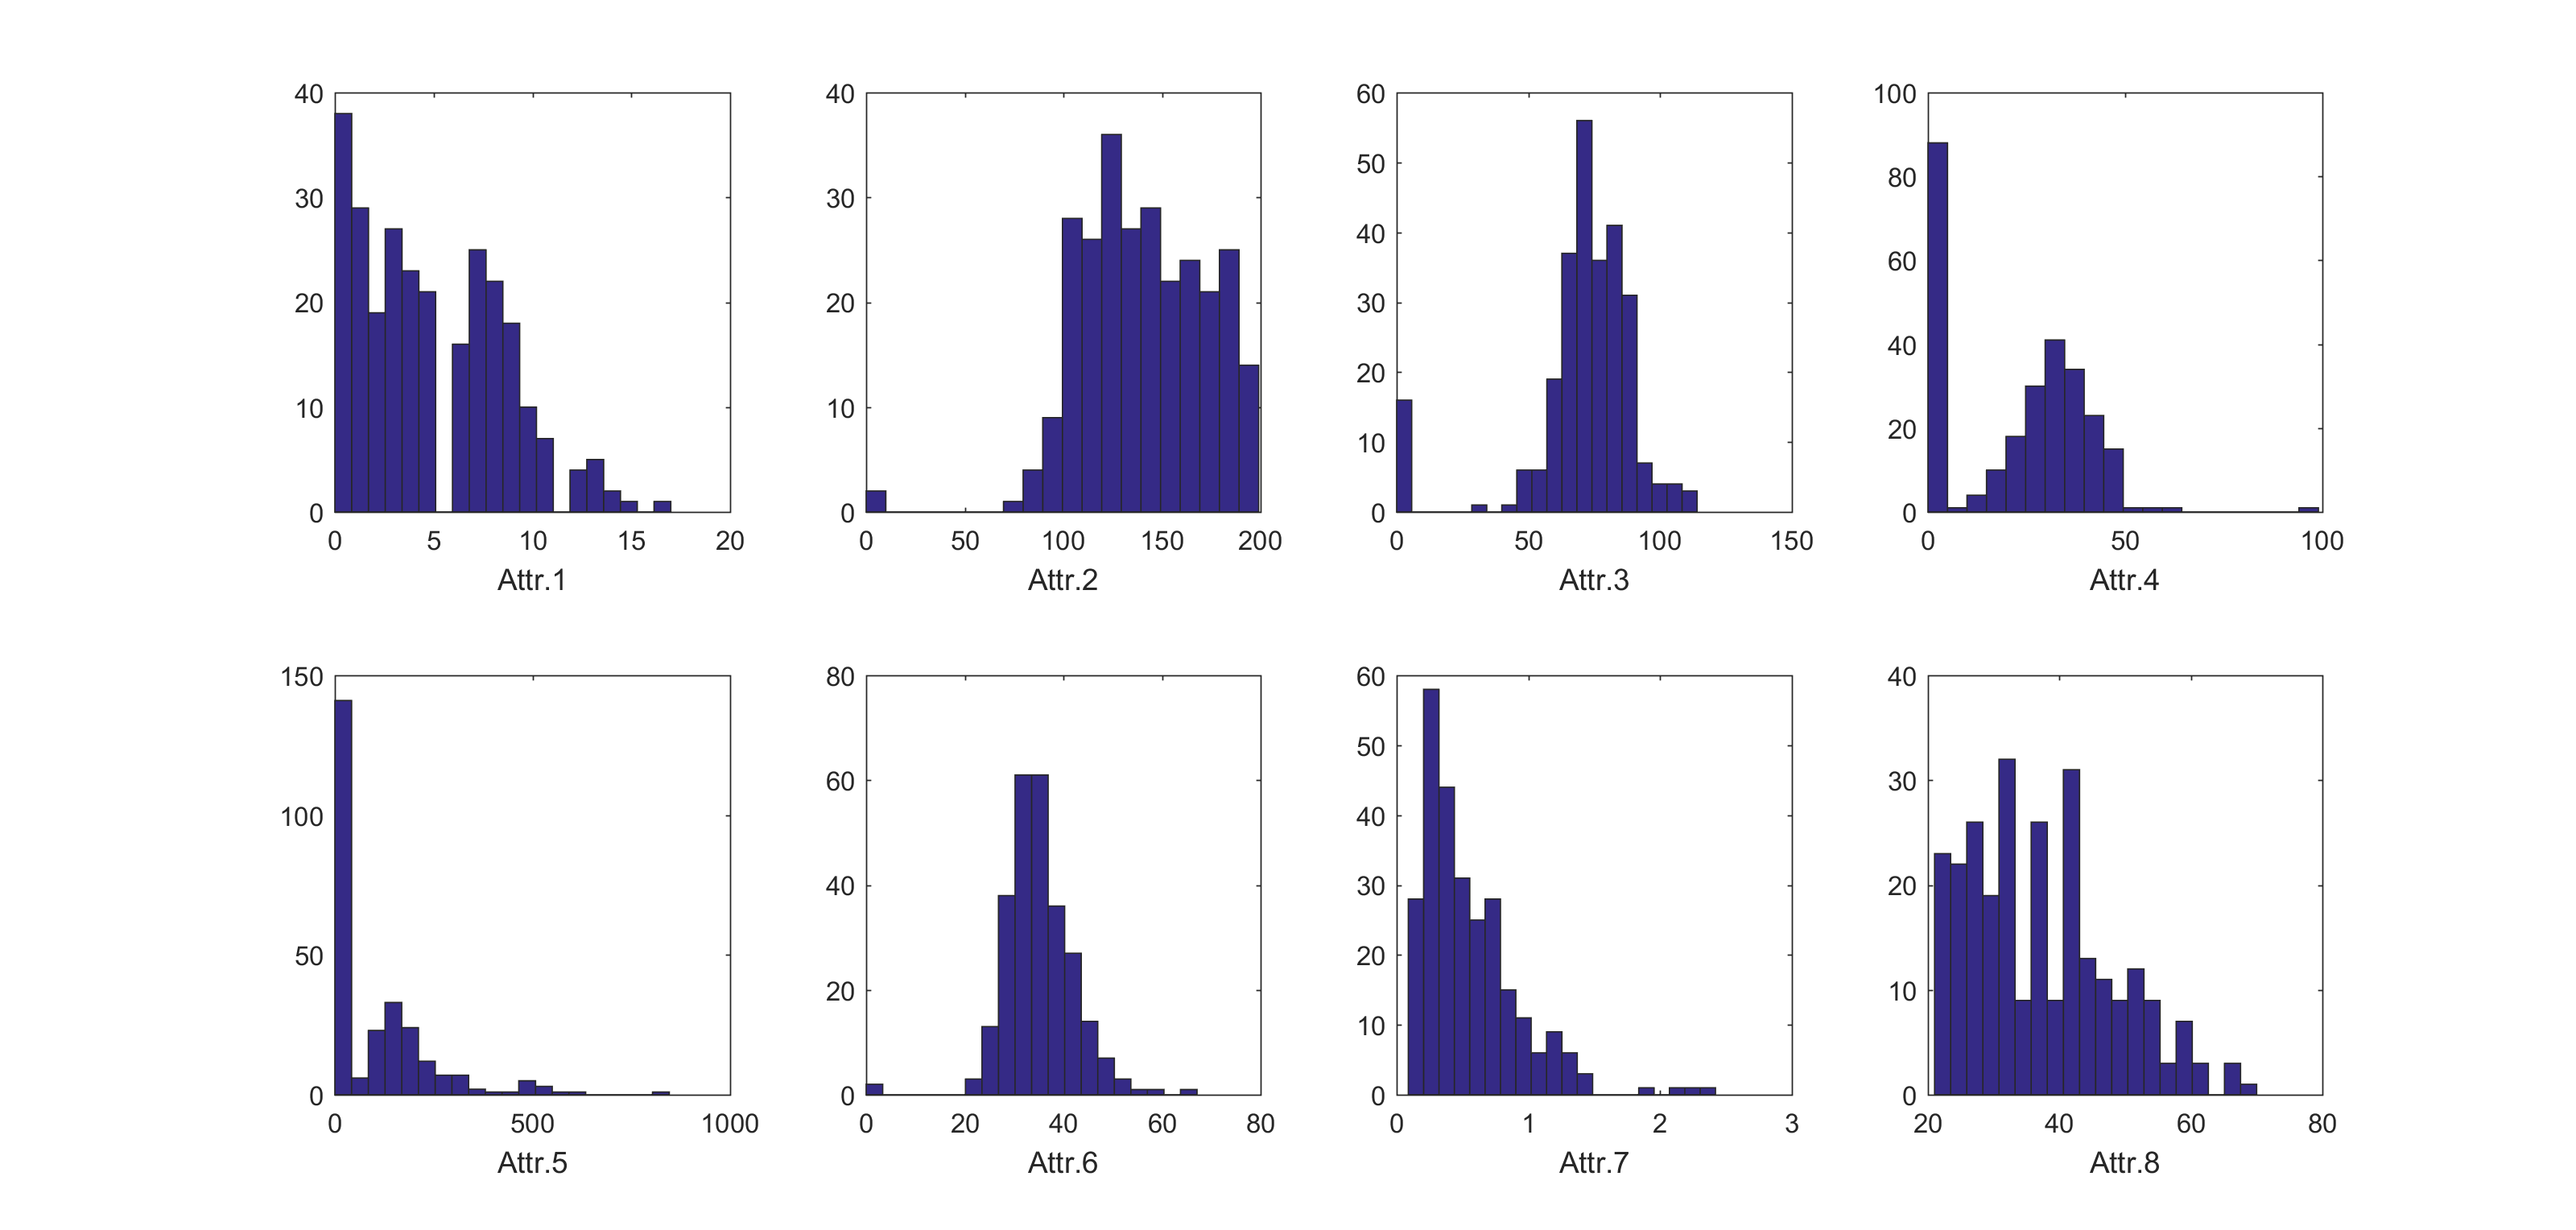
\includegraphics[width=\columnwidth]{p2a1.png}
	\caption{Class 1}
\end{figure}

% B
\subsection{Data Distribution}

\begin{table}[H]
	\centering
	\begin{tabular}{ |l|l| }
		\hline
		\textbf{Attribute} & \textbf{Distribution} \\
		\hline
		1 & Exponential \\
		\hline
		2 & Normal \\
		\hline
		3 & Normal \\
		\hline
		4 & Normal \\
		\hline
		5 & Exponential\\
		\hline
		6 & Normal \\
		\hline
		7 & Exponential \\
		\hline
		8 & Exponential \\
		\hline
	\end{tabular}
	\caption{Attribute Distribution}
\end{table}

\section{Problem 2.2 - Naive Bayes Learning}

% A
\subsection{Naive Bayes Training Data}

\begin{verbatim}
    main2_2.m
\end{verbatim}

% B
\subsection{Naive Bayes Parameters}

\begin{table}[H]
	\centering
	\begin{tabular}{ |l|l|l|l|l|l|l| }
		\hline
		\textbf{Attribute} & \textbf{$\mu$} & \textbf{$\sigma$} & \textbf{CI $\mu$ lower} & \textbf{CI $\mu$ upper} & \textbf{CI $\sigma$ lower} & \textbf{CI $\sigma$ upper} \\
		\hline
		2 & 109.98 & 26.1412 & 107.6831 & 112.2769 & 24.6152 & 27.8705 \\
		\hline
		3 & 68.184 & 18.0621 & 66.5969 & 69.7711 & 17.0086 & 19.258 \\
		\hline
		4 & 19.664 & 14.8899 & 18.3557 & 20.9723 & 14.020 & 15.8749 \\
		\hline
		6 & 30.3042 & 7.6899 & 29.6285 & 30.9799 & 7.2409 & 8.1986 \\
		\hline
	\end{tabular}
	\caption{Class 0 Normal}
\end{table}

\begin{table}[H]
	\centering
	\begin{tabular}{ |l|l|l|l|l|l|l| }
		\hline
		\textbf{Attribute} & \textbf{$\mu$} & \textbf{$\sigma$} & \textbf{CI $\mu$ lower} & \textbf{CI $\mu$ upper} & \textbf{CI $\sigma$ lower} & \textbf{CI $\sigma$ upper} \\
		\hline
		2 & 141.2575 & 31.9396 & 137.4161 & 145.0988 & 29.4451 & 34.8995 \\
		\hline
		3 & 70.8246 & 21.4918 & 68.2398 & 73.4094 & 19.8133 & 23.4835 \\
		\hline
		4 & 22.1642 & 17.6797 & 20.0379 & 24.2905 & 16.2989 & 19.3181 \\
		\hline
		6 & 35.1425 & 7.2630 & 34.269 & 36.0160 & 6.6957 & 7.9360 \\
		\hline
	\end{tabular}
	\caption{Class 1 Normal}
\end{table}

\begin{table}[H]
	\centering
	\begin{tabular}{ |l|l|l|l|l }
		\hline
		\textbf{Attribute} & \textbf{$\mu$} & \textbf{CI $\mu$ lower} & \textbf{CI $\mu$ upper} \\
		\hline
		1 & 3.2980 & 3.0270 & 3.6073 \\
		\hline
		5 & 68.792 & 63.139 & 75.2436 \\
		\hline
		7 & 0.4297 & 0.3944 & 0.4700 \\
		\hline
		8 & 31.190 & 28.627 & 34.1151 \\
		\hline
	\end{tabular}
	\caption{Class 0 Exponential}
\end{table}

\begin{table}[H]
	\centering
	\begin{tabular}{ |l|l|l|l|l }
		\hline
		\textbf{Attribute} & \textbf{$\mu$} & \textbf{CI $\mu$ lower} & \textbf{CI $\mu$ upper} \\
		\hline
		1 & 4.8657 & 4.3319 & 5.5051 \\
		\hline
		5 & 100.3358 & 89.3289 & 113.5215 \\
		\hline
		7 & 0.5505 & 0.4901 & 0.6228 \\
		\hline
		8 & 37.0672 & 33.0009 & 41.9384 \\
		\hline
	\end{tabular}
	\caption{Class 1 Exponential}
\end{table}

\section{Problem 2.3 - Naive Bayes Classification}

% A
\subsection{NB Prediction}

\begin{verbatim}
    main2_3.m
\end{verbatim}

% B
\subsection{Misclassification, Confusion, Sensitivity, Specificity}

\begin{table}[H]
	\centering
	\begin{tabular}{ |l|l| }
		\hline
		\textbf{Dataset} & \textbf{Misclassification Error} \\
		\hline
		Training & 0.5356 \\
		\hline
		Testing & 0.6241 \\
		\hline
	\end{tabular}
	\caption{Misclassification Error}
\end{table}

\begin{table}[H]
	\centering
	\begin{tabular}{ |r|l|l| }
		\hline
		\textbf{Predict / Target} & \textbf{1} & \textbf{1} \\
		\hline
		\textbf{1} & 168 & 156 \\
		\hline
		\textbf{0} & 32 & 183 \\
		\hline
	\end{tabular}
	\caption{Training Confusion Matrix}
\end{table}

\begin{table}[H]
	\centering
	\begin{tabular}{ |r|l|l| }
		\hline
		\textbf{Predict / Target} & \textbf{1} & \textbf{1} \\
		\hline
		\textbf{1} & 59 & 79 \\
		\hline
		\textbf{0} & 9 & 82 \\
		\hline
	\end{tabular}
	\caption{Test Confusion Matrix}
\end{table}

\begin{table}[H]
	\centering
	\begin{tabular}{ |l|l| }
		\hline
		Sensitivity & 0.8676 \\
		\hline
		Specificity & 0.5093 \\
		\hline
	\end{tabular}
	\caption{Test Sensitivity / Specificity}
\end{table}


% C
\subsection{Logistic Regression vs. Naive Bayes}

\begin{table}[H]
	\centering
	\begin{tabular}{ |l|l|l| }
		\hline
		\textbf{Model} & \textbf{Training} & \textbf{Testing} \\
		\hline
		Logistic Regression & 0.2988 & 0.2722 \\
		\hline
		Naive Bayes & 0.5356 & 0.6241 \\
		\hline
	\end{tabular}
	\caption{Misclassification Error}
\end{table}

\section{Problem 3 - ROC Analysis}

% A
\subsection{\textit{perfcurve()}}

Receiver operating characteristic (ROC) curve or other performance curve for classifier output.

% B
\subsection{ROC}

\begin{verbatim}
    roc_analysis.m
\end{verbatim}


% C
\subsection{AUC}

\begin{figure}[H]
	\captionsetup[subfigure]{labelformat=empty}
	\centering
	\subfloat[Figure 3]{{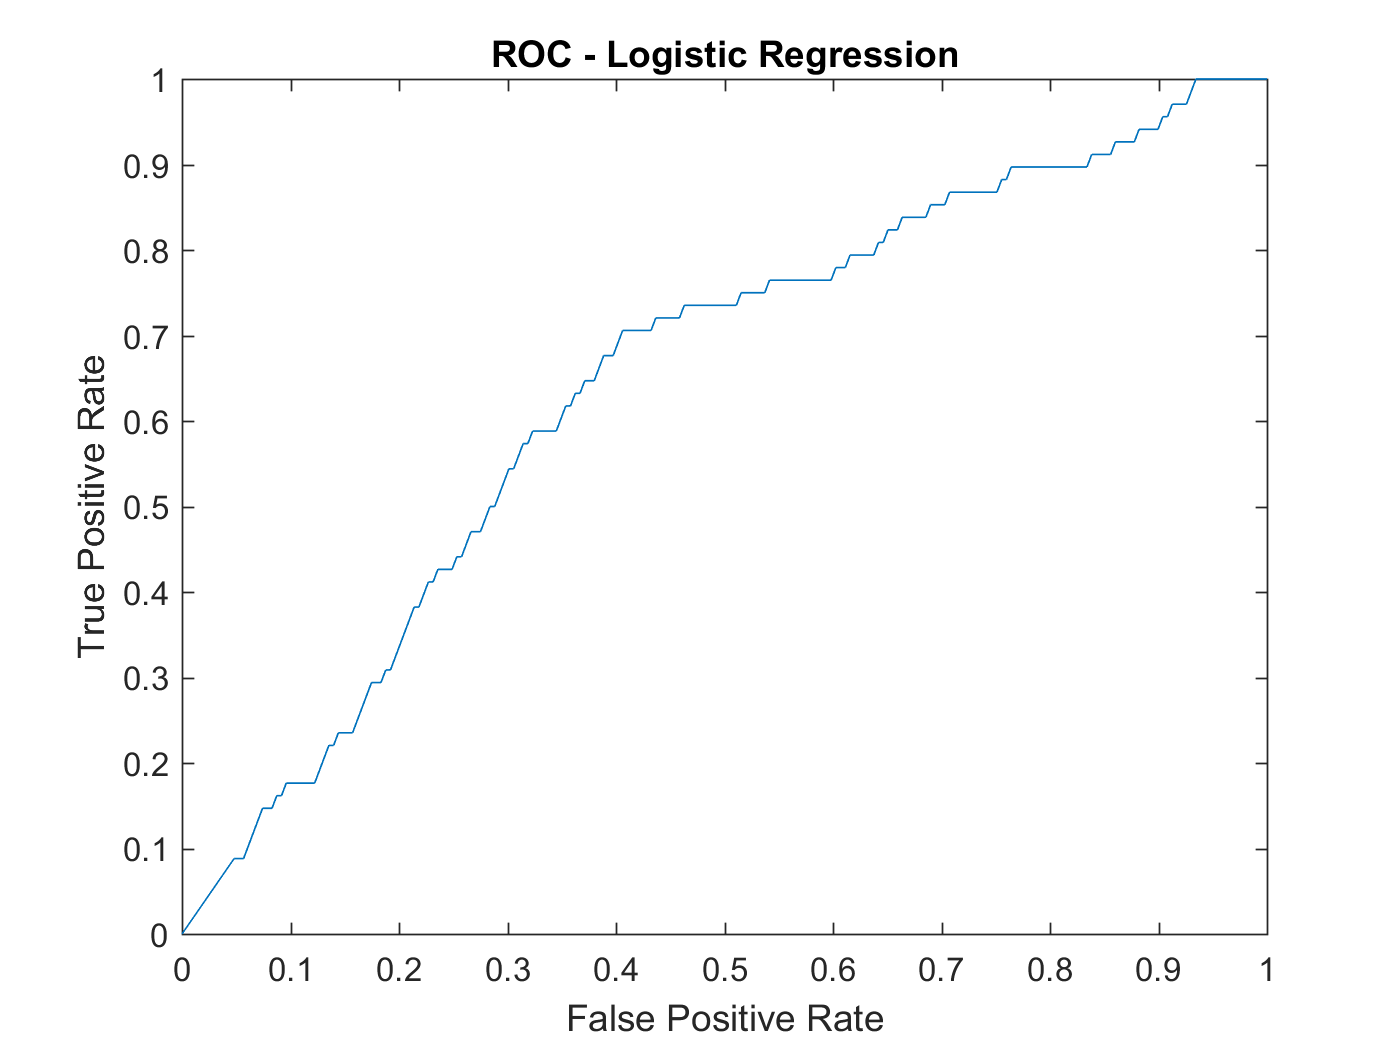
\includegraphics[width=18em]{p3lr.png} }}
	\qquad
	\subfloat[Figure 4]{{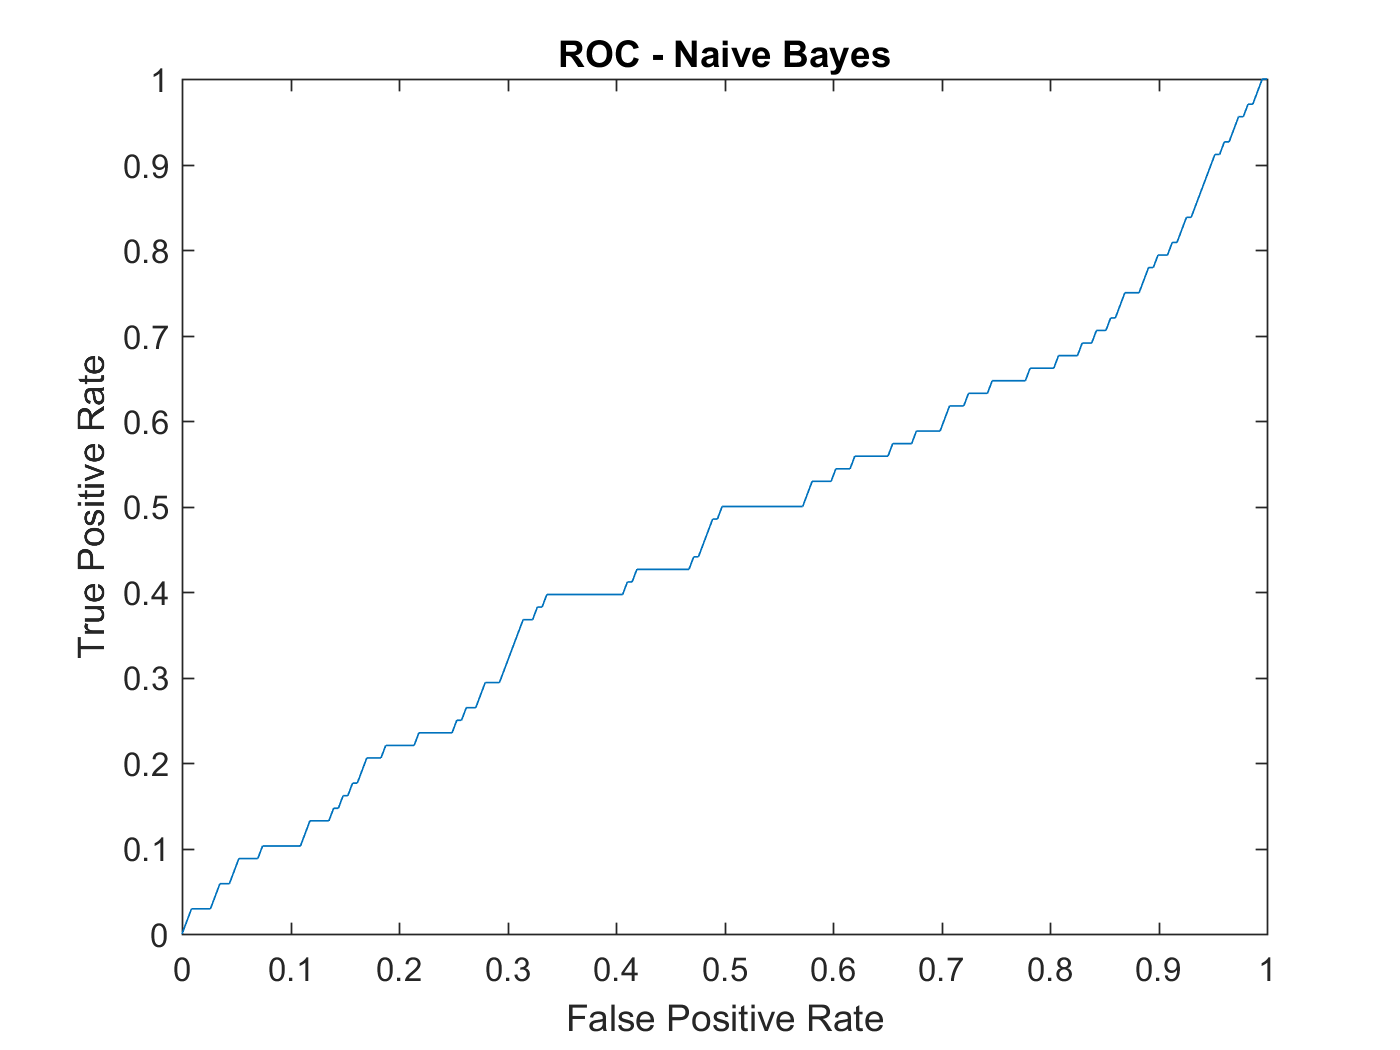
\includegraphics[width=18em]{p3nb.png} }}
	\label{fig:example}
\end{figure}

\begin{table}[H]
	\centering
	\begin{tabular}{ |l|l| }
		\hline
		\textbf{Model} & \textbf{AUC} \\
		\hline
		Logistic Regression & 0.8518 \\
		\hline
		Naive Bayes & 0.4450 \\
		\hline
	\end{tabular}
	\caption{AUC}
\end{table}

Based on the collected data for the ROC curves and the AUC statistics, logistic regression outperforms the Naive Bayes implementation, with a higher true positive rate and AUC.


\end{document}